\documentclass{article}
\usepackage{graphicx}
\usepackage{url}
\usepackage[backend=biber]{biblatex}
\addbibresource{sample.bib}

\begin{document}

\newcommand{\HRule}{\rule{\linewidth}{0.5mm}} 
\begin{titlepage}

\center

\textsc{\LARGE COLLEGE OF ENGINEERING }\\[1.3cm]
\textsc{\Large TRIVANDRUM}\\[0.5cm]

\HRule \\[0.4cm]
{ \huge \bfseries FOSS LAB RECORD}\\[0.4cm] 
\HRule \\[1.5cm]




\begin{minipage}{0.4\textwidth}
\begin{flushleft} \large
\emph{Submitted By:}\\


 \textsc{Santhisenan A \\
 Roll Number 50 \\
 S4 CSE\\
 } 
\end{flushleft}
\end{minipage}
~
\begin{minipage}{0.4\textwidth}
\begin{flushright} \large
\emph{} \\
\end{flushright}
\end{minipage}\\[4cm]


{\large \today}\\[3cm] 


\vfill



\end{titlepage}
\newpage
\tableofcontents{}
%\makeindex

\newpage
\section{Getting started with Linux basic commands for directory operations}

\subsection{Aim}
Getting started with Linux basic commands for directory operations, displaying directory structure in tree format etc.

\subsection{Basic Commands}
\begin{table}[htb]
\caption{Basic Commands}

\label{Basic commands in Linux}
\begin{tabular}{rcc}
\noalign{\smallskip} \hline \hline \noalign{\smallskip}
Command & operation \\

\hline
touch filename        	& create a new file\\
mkdir filename			&create a new directory\\
pwd						&prints present working directory\\
cd dirname				&change directory\\
\hline
cat filename	&view contents of a file\\
more filename	&view contents of a file one scornful at a time\\
less filename 	&similar but faster than more\\
\hline
ls				&list files in a directory\\
ls -l 			&provide long listing of all the files\\
ls -l -h		&provides sizes in human readable form\\
ls -F			&mark all executables with * and directories with / \\
ls -a			&show all files in the present directory with special dot files\\
\hline
cp file1 file2			&copying files\\
cp -r dirname1 dirname2	&copy directories\\
\hline
rm filename			&remove a file\\
rmdir -rf dirname	&remove a non empty directory\\
\hline
clear			&clear the contents of the terminal\\
locate			&search for a specified filename\\
man commandname	&view help of the specified command name\\
\hline
chmod [options] mode filename &change file permissions\\
chwon [options] filename &Change file ownership\\
kill [options] pid &Kill a process\\
who [options] &Display who is logged in\\
top &Display the resources being used in your system\\
ln [options] source [desitination] &Create a shortcut\\
\noalign{\smallskip} \hline \noalign{\smallskip}
\end{tabular}
\end{table}

\newpage

\subsection{Directory Structure in Linux}
\begin{table}[htb]
\caption{Directory structure}
\label{Directory Structure in Linux}
\begin{tabular}{rcc}
\noalign{\smallskip} \hline \hline \noalign{\smallskip}
File name & Content\\
/bin & Essential user command binaries\\
/boot & Static files and boot loader\\
/dev & Device files\\
/etc & Host specific system configuration\\
/home & User home directories\\
/lib & Essential shared libraries and kernel modules\\
/mnt & Mount point for devices\\
/opt & Add on application software packages\\
/sbin & System binaries\\
/tmp & Temporary files\\
/usr & User utilities and applications\\
/var &variable files\\
/root & home directory for the root user\\ 
\hline
\noalign{\smallskip} \hline \noalign{\smallskip}
\end{tabular}
\end{table}


\subsection{Output}
\begin{figure}[h!]
	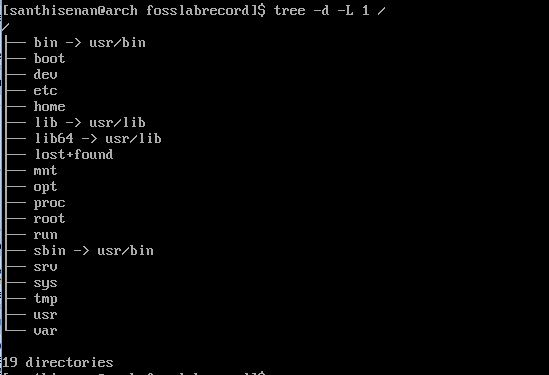
\includegraphics[width=\linewidth]{./outputs/exp1.jpg}
\end{figure}

\subsection{Result}
Several basic linux commands were studied and they were tested on OS version number. The direcotry structure of linux was also studied. The directory structure was printed in tree format using tree command on ArchLinux 4.10.11. A more detailed directory struture in tree format can be found in this file - \url{https://github.com/santhisenan/fosslabrecord/blob/master/exp4out}
\begin{refsection}
\cite{commands}
\cite{directorystructure}
\printbibliography
\end{refsection}
%Second Experiment
\newpage
\section{Linux commands for operations such as redirection, pipes, filters, job control, changing ownership/permissions of files/links/directory.}

\subsection{Aim}
Linux commands for operations such as redirection, pipes, filters, job control, changing ownership/permissions of files/links/directory.

\subsection{Redirection of standard Input/Output}
\begin{itemize}
\item By default most command line programs send their output to the standard output which by default displays it on the 

\hspace{10mm} \textit{commandName} $>$\textit{fileName} -Overwrites the file with the output of the command

\hspace{10mm} \textit{commandName} $>>$\textit{fileName} - appends the file with the output of the command.

\item Most of the command line programs accept its input from the standard input and by default gets its contents from the keyboard. Similar to standard output it can also be redirected.

\textit{sort $<$ filename} - sort command processes the contents of the file with the name filename.

\hspace{10mm} \textit{sort $<$ file1 $>$ file2} processes the contents of file 1 and redirects its output to file 2

\end{itemize}

\subsection{Pipes}
Pipes are used to redirect the standard output of one command to the standard input of another command.

\hspace{10mm} \textit{command1 $|$ command2} the standard output of command 1 is redirected to the standard input of command 2.

\subsection{Filters}

Filters take the standard input and perform an operation upon it and sends the results to the standard output. This can be used to process information in powerful ways.
\begin{itemize}
\item \textit{sort} - sorts the standard input and sends the output to standard output.

\hspace{10mm} `sort filename' rearranges each line of file in alphabetical order and outputs it to the standard output.

\item \textit{uniq} - Given a sorted stream of data from standard input it removes the duplicate lines of data and returns the result to the standard output.

\item \textit{grep} - examines each line of data it receives from standard input and outputs all lines that contains a specific pattern of characters.

\hspace{10mm} `grep ``string" new.txt' outputs lines of text in new.txt which contain the word string.

\item \textit{fmt} - reads text from standard input and outputs formatted text to standard output.

\hspace{10mm} `fmt filename' formats contents of filename and outputs it in standard output.

\item \textit{pr} - Takes data from the standard input and splits the data into pages with page breaks, footers and headers in preparation for printing.

\hspace{10mm} `pr filename' displays the contents of the file one page after the other and returns the output to the standard output.

\item \textit{head} - Outputs the first few lines of the file and returns it to the standard output.

\item \textit{tail} - Outputs the last few lines of the file and returns it to the standard output.

\item \textit{tr} - Translates Characters. Can be used to perform tasks such as uppercase to lowercase conversions or changing the line termination characters from one type to another.

\hspace{10mm} `tr [:lower:] [:upper:]' takes input from the keyboard and outputs each character of the input to uppercase characters and outputs it to the standard output.

\end{itemize}

\subsection{Job Control}
There are several commands used to control processes in Linux.
\begin{itemize}
\item \textit{ps} - The ps commands lists the processes running in the system.

\hspace{10mm} `ps lists' all processes running in the system

\hspace{10mm} `ps aux' lists all processes running in the system

\item \textit{kill} - sends a signal to the specified processes usually to stop the execution of the processes.
\hspace{10mm} `kill -l' lists the signal names that can be sent to processes in Linux.

\hspace{10mm} `kill pid' to kill the processes specified by the process id (pid) which can be obtained by the ps command.

\hspace{10mm} `kill -s SIGKILL pid' is used to send SIGKILL signal to process with process id `pid'. This command is used to forcefully kill a process without memory cleanup.

\hspace{10mm} A signal is an asynchronous notification sent to a process or to a specific thread within the same process in order to notify it of an event that occurred.

\item \textit{jobs} -  An alternate way of listing the processes. jobs is a shell builtin command which gives you information internal to the shell such as the job numbers.

\hspace{10mm} `jobs' lists the jobs that the current shell is managing.

\item \textit{bg} - used to put a process in background.

\item \textit{fg} - used to put a process in foreground

\end{itemize}

\subsection{Permissions}

\begin{table}[htb]
\caption{Permissions}
\label {Permissions}
\begin{tabular}{rcc}
\noalign{\smallskip} \hline\hline \noalign{\smallskip}
chmod & modify file access rights\\
su & temporarily become super user\\
chown & change file ownership\\
chgrp & change file group ownership\\
\noalign{\smallskip} \hline\hline \noalign{\smallskip}
\end{tabular}
\end{table}

\subsection{Links}

A link provides a connection between files. This provides the ability to have a single file or directory referred to through different names.

	The nearest comparison with the Windows world is of a shortcut, but that is an unfair comparison as a link in Linux is far more powerful. A Windows shortcut is just a way of launching a file from a different place, whereas a link can make a file appear in multiple locations which is invisible to the applications.

	There are two types of links that can be created. The first is a hard link and the other is a soft link (sometimes called symbolic link or symlink). The command to create these is the same - ln.
	
\begin{itemize}
\item Hard Link
A hard link creates a second file that refers to the same file on the physical disk. This is achieved by having two filenames that point directly at the same file. This is normally used where file entries (links) are on the same filesystem. When a hard link is created then all the names that link to that file are given the same status. Deleting one of the files will break the link, but the file can still exist under the other linked filenames. This works by maintaining a counter of the number of filenames that the file has. When the number of filenames reaches zero then the file is considered to be deleted and is removed.

	The number of filenames for a file can be seen using the `ls -l' command. The number following the file permissions indicates the number of linked filenames. The following screenshot shows that filename1 and filename2 are to linked files with one of the file denoted by the 2 (in this case the same file, but they could be to completely different files), the file not\_link is a single file denoted by the 1.
\begin{verbatim}	
ls -l

total 2432

-rw-r--r-- 2 stewart stewart 1241088 2009-01-23 15:26 filename1

-rw-r--r-- 2 stewart stewart 1241088 2009-01-23 15:26 filename2

-rw-r--r-- 1 stewart stewart       0 2009-01-23 15:26 not\_link

Note that whilst the two files appear to occupy 1.2Mb each the actual space used is only 1.2Mb in total as the file only exists once.

du -h

1.2M

The default for the ln command is a hard link. Assuming filename1 already exists filename2 is created using:

ln filename1 filename2

\end{verbatim}

\item Soft Link

A soft link is sometimes referred to as a symbolic link or symlink. A filename created as a soft link is a special file that has the pathname of the file to redirect to. Behind the scenes when you try and access a symlink it just goes to the filename referred to instead.

	In the following example a file has been created called original\_file with a soft link to that same file called softlink\_tofile. As you can see the ls command makes it clear that this is a link through the l at the beginning of the file permissions and due to the reference notation after the filename.
\begin{verbatim}
ls -l

total 440

-rw-r--r-- 1 stewart stewart 446464 2009-01-23 15:21 original_file

lrwxrwxrwx 1 stewart stewart     13 2009-01-23 15:20 softlink_tofile -> original_file

Note that with a soft link the permissions to the link file are set to full access as the user is contstrained by the permissions on the original file. Also note that if the filesize of the original file changes the link will remain the same (on this system 13 bytes).

If the link is deleted then this will have no impact on the original file, but if the original file is deleted this will result in a broken link. The example below shows how removing the original file results in a error "No such file or directory".

$ rm original_file 

$ ls -l

total 0

lrwxrwxrwx 1 stewart stewart 13 2009-01-23 15:20 softlink_tofile -> original_file

$ cat softlink_tofile 

cat: softlink_tofile: No such file or directory

The -s option is used on the ln command to create a softlink.

ln -s original_file softlink_tofile
\end{verbatim}
\hspace{10mm}Note that if original\_file does not exist then the soft link will be created anyway. An attempt to read it will give the error message we encountered earlier, but an attempt to write to the file can create original\_file.

\item Pitfalls while using links

\begin{itemize}
\item There are some things that you need to be aware of, particularly when using softlinks.

\item Some programs (e.g. Apache) can be configured to not follow soft links (from a security 

\item When creating backup files you need to be aware of how the particular backup program / tool 

\item Using one method the program may not backup the file referenced resulting in an incomplete backup of the 

\item Using another method the program may end up backing up both as individual files using double the space for that 

\item Using the second method of the above could result in the file being restored as a real file rather than as a link, breaking their connection

\item The original file could be deleted without realising that there are other symlinked files referring to it

Despite these pitfalls there are many advantages to using both hard and soft links to provide multiple references to files.
				
\end{itemize}
\end{itemize}


\subsection {Result}

The required linux commands were studied.

\begin{refsection}
\cite{jobcontrol}
\cite{piperedirection}
\cite{linuxbook}
\printbibliography
\end{refsection}
\newpage
\section{Advanced Linux Commands}

\subsection{Aim}
Advanced linux commands curl, wget, ftp, ssh and grep.

\subsection{curl}

curl \cite{curlweb} is a tool to transfer data from or to a server, using one of the supported protocols (DICT, FILE, FTP, FTPS, GOPHER, HTTP, HTTPS, IMAP, IMAPS, LDAP, LDAPS, POP3, POP3S, RTMP, RTSP, SCP, SFTP, SMB, SMBS, SMTP, SMTPS, TELNET and TFTP). The command is designed to work without user interaction.

`curl link' - gives information about the website and outputs the html code.

`curl -O link/file.html' - copies the html code of the website to file.html

\subsection{ssh}

     ssh (SSH client) is a program for logging into a remote machine and for
     executing commands on a remote machine.  It is intended to replace rlogin
     and rsh, and provide secure encrypted communications between two
     untrusted hosts over an insecure network.  X11 connections and arbitrary
     TCP/IP ports can also be forwarded over the secure channel.

     ssh connects and logs into the specified hostname (with optional user
     name).  The user must prove his/her identity to the remote machine using
     one of several methods depending on the protocol version used.

     If command is specified, command is executed on the remote host instead
     of a login shell.
    
BASIC COMMAND

\begin{verbatim}
$ ssh remote_host
\end{verbatim}
\hspace{10mm}The remote\_host in this example is the IP address or domain name that you are trying to connect to.
If your username is different on the remote system, you can specify it by using this syntax:
\begin{verbatim}
$ ssh remote_username@remote_host
\end{verbatim}

TO COPY FILES
\begin{verbatim}
$ scp source destination
\end{verbatim}

COPY A FILE FROM HOST TO LOCAL

\begin{verbatim}
$ scp localhostfile.txt jsmith@remotehost.example.com:/home/jsmith/localhostfile.txt
\end{verbatim}

COPY A FILE FROM LOCAL TO HOST
\begin{verbatim}
$ scp localhostfile.txt jsmith@remotehost.example.com:/home/jsmith/localhostfile.txt
\end{verbatim}

TO SHUTDOWN CONNECTED COMPUTER 
		\begin{verbatim}

		$ ssh user@remote\_computer
		
		$ sudo poweroff
		
		$ sudo reboot 
		
		\end{verbatim}


\subsection{wget}


GNU wget \cite{wgetweb} is a free utility for non-interactive download of files from the Web. It supports HTTP , HTTPS , and FTP protocols, as well as retrieval through HTTP proxies.

Wget is non-interactive, meaning that it can work in the background, while the user is not logged on. This allows you to start a retrieval and disconnect from the system, letting Wget finish the work. By contrast, most of the Web browsers require constant user's presence, which can be a great hindrance when transferring a lot of data.

Wget can follow links in HTML , XHTML , and CSS pages, to create local versions of remote web sites, fully recreating the directory structure of the original site. This is sometimes referred to as "recursive downloading." While doing that, Wget respects the Robot Exclusion Standard (/robots.txt). Wget can be instructed to convert the links in downloaded files to point at the local files, for offline viewing.

Wget has been designed for robustness over slow or unstable network connections; if a download fails due to a network problem, it will keep retrying until the whole file has been retrieved. If the server supports regetting, it will instruct the server to continue the download from where it left off.

\hspace{10mm} \textit{wget http://www.openss7.org/repos/tarballs/strx25-0.9.2.1.tar.bz2} this command will download a single file and store it in the current repository.

\hspace{10mm} \textit{wget -O wget.zip http://ftp.gnu.org/gnu/wget/wget-1.5.3.tar.gz} Using -O (uppercase) option, downloads file with different file name. Here we have given wget.zip file name as show below.

\hspace{10mm} \textit {wget -c http://www.openss7.org/repos/tarballs/strx25-0.9.2.1.tar.bz2} Restart a download which got stopped in the middle using wget -c option.

\hspace{10mm} \textit{wget --mirror [WebsiteName]} If you wish to retain a copy of any website that you may like to refer to/read locally, or maybe save a copy of your blog to the hard disk as back up, you may execute the wget command with mirror option.

\hspace{10mm} \textit{wget -i download-file-list.txt} allows you to download multiple files stored in download-file-list.txt simultaneously.



\newpage

\subsection {ftp}

The FTP \cite{ftpweb1} \cite{ftpweb2} (File Transfer Protocol) utility program is commonly used for copying files to and from other computers. These computers may be at the same site or at different sites thousands of miles apart. FTP is a general protocol that works on UNIX systems as well as a variety of other (non-UNIX) systems.

To connect your local machine to the remote machine, type

\hspace{10mm} ftp machinename

where machinename is the full machine name of the remote machine, e.g., some-url.com. If the name of the machine is unknown, you may type

\hspace{10mm}ftp IP-Address

where machinennumber is the net address of the remote machine, e.g., 129.82.45.181. In either case, this command is similar to logging onto the remote machine. If the remote machine has been reached successfully, FTP responds by asking for a loginname and password.

When you enter your own loginname and password for the remote machine, it returns the prompt

\hspace{10mm}ftp $>$

and permits you access to your own home directory on the remote machine. You should be able to move around in your own directory and to copy files to and from your local machine using the FTP interface commands.

\begin{table}[htb]
\caption {FTP Interface Commands}
\label {Common Commands}
\begin{tabular}{rcc}
\noalign{\smallskip}\hline\hline\noalign{\smallskip}
? & request help or information about FTP Commands\\
cd & change directory in remote machine\\
close & terminate a connection with remote computer\\
delete & delete a file in remote computer\\
get & get a copy of a file in the remote machine to local machine\\
ls & list the names of files in the current directory in the remote machine\\
mkdir & make a new directory in the remote machine\\
pwd & print the working directory in remote machine\\
quit & exit ftp environment\\
\noalign{\smallskip}\hline\hline\noalign{\smallskip}

\end{tabular}
\end{table}

\subsection{grep}

GREP : Global Regular Expression Print \cite{grepweb}

 	\hspace{10mm}Searches for text in a file
	
 	\hspace{10mm}Can search for simple words.
	
 	\hspace{10mm}Can look for regular expression - more complex charecter strings( words followed by any no of spaces, followed by a digit or lowercase letter).


	Searching the given string

		     \hspace{10mm}`\$ grep $<$literal\_string$>$ ' filename To search a specific string in a specified file


	Case insensitive search
	
			        \hspace{10mm}\$ grep -i ?string? filename
			        
       				\hspace{10mm}\$ grep -i ?string? FILE\_PATTERN\*
				
				\hspace{10mm}-This searches for given string/pattern case insensitively.


	Simple regular expressions

				\hspace{10mm}?[0-9]? look for any digit



				\hspace{10mm}?[a-zA-Z]? look for one upper or lower case letter	


				\hspace{10mm}?.? look for one charector
				
				\hspace{10mm}?.*? any number of charectors
				
				\hspace{10mm} ?$\backslash$.? a literal decimal point
				
				\hspace{10mm}?$\backslash$.161:? dot, then 161, then colon 
				
				\hspace{10mm}?$\backslash$.161[: ]? dot, then 161, then colon or space	


	Advanced regular expressions

				\hspace{10mm}Look for lines that hold either string1 or string2
				
				\hspace{10mm}\$ grep -E ?(string1|string2)? filename 
				
				\hspace{10mm}Lines that have string1 followed by string2 on the same line, but possibly with other charectors in between.
				
				\hspace{10mm}\$ grep ?string1.*string2? filename	
				
				\hspace{10mm}String1 has to be at the beginning of the line.
				
				\hspace{10mm}\$ grep ?\^string1? filename
				
				Look for it at the end of the line.
				
				\hspace{10mm}\$ grep ?string1\$? filename

\subsection{Output}
\newpage
\begin{figure}[!h]
	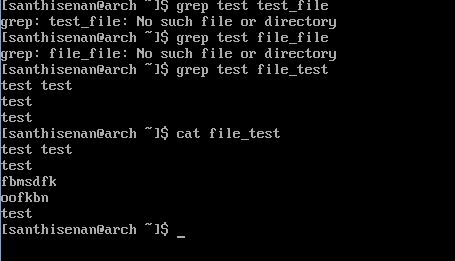
\includegraphics[width=\linewidth]{./outputs/advlin1.jpg}
	\bigskip
	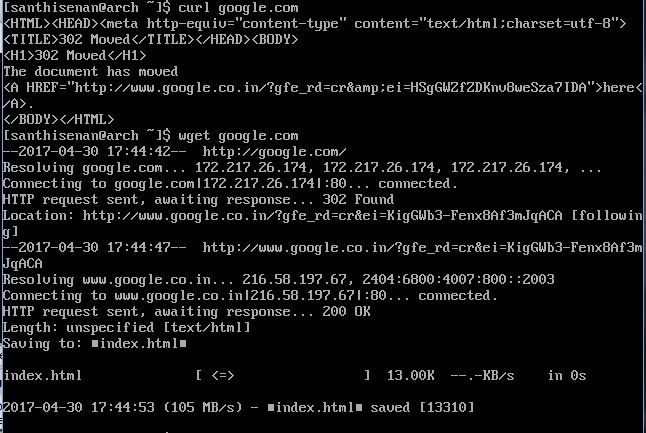
\includegraphics[width=\linewidth]{./outputs/advlinux.jpg}
\end{figure}	
\newpage

\subsection{Result}
The advanced linux commands ftp, ssh, wget, grep and curl were studied. The commads were run on ArchLinux 4.10.11.

\begin{refsection}
\cite{ftpweb1}
\cite{ftpweb2}
\cite{curlweb}
\cite{wgetweb}
\cite{grepweb}
\printbibliography

\end{refsection}

\newpage

\section{Shell Programming}
\subsection{Aim}
Write shell script to show various system configuration like
\begin{itemize}
\item Currently logged user and his login name
\item Your current shell
\item Your home directory
\item Your operating system type
\item Your current path setting
\item Your current working directory
\item Number of users currently logged in
\end{itemize}

\subsection{Shell Script}
\begin{verbatim}
clear
log=`who|wc -l`
echo "the currently logged in user is $USER"
echo "the current shell is $SHELL"

echo "the home drectory is  $HOME"

echo "the os type  is $OSTYPE"
echo "the current path setting is $PATH"
echo "the working directory is $PWD"
echo "there are $log users logged in"
\end{verbatim}

\subsection{Output}
\begin{figure}[h!]
	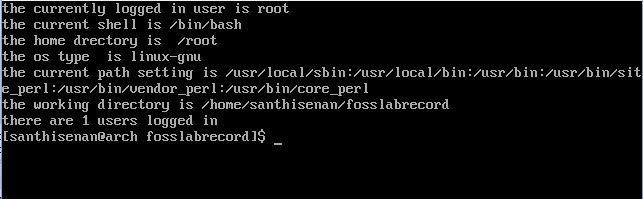
\includegraphics[width=\linewidth]{./outputs/exp3new.jpg}
\end{figure}

\subsection{Result}
The shell script for displaying various system configurations were made and the output was verified. The script was run on ArchLinux 4.10.11.
\begin{refsection}
\cite{shellbible}
\cite{shellbook}
\printbibliography
\end{refsection}

\newpage

\newpage

\section{Shell script to show various system configurations}

\subsection {Aim}

Write shell script to show various system configurations like
\begin{itemize}
\item your OS and version, release number, kernel version
\item all available shells
\item computer CPU information like processor type, speed etc
\item memory information
\item hard disk information like size of hard-disk, cache memory, model etc
\item File system (Mounted)
\end{itemize}

\subsection{Shell Script}

\begin{verbatim}

  \#!/bin/bash
   
  echo -e "`cat /etc/os-release`"
  echo -e  "`cat /etc/shells`"
  echo -e "`xset q`"
  echo -e "`cat /proc/meminfo`"
  echo -e "Driver: `sudo hdparm -I /dev/sda`"
  echo -e "`cat /proc/mounts`"

\end{verbatim}

\subsection{Result}
The shell script for displaying required system configurations was made and the output was verified. The shell script was run on ArchLinux 4.10.11 and the output file can be viewed at \url{https://github.com/santhisenan/fosslabrecord/blob/master/exp4out}

\begin{refsection}
\cite{shellbible}
\cite{shellbook}
\printbibliography
\end{refsection}

\newpage

\section{Menu driven calculator}
\subsection{Aim}
Write a shell script to implement a menu driven calculator with following functions
\begin{itemize}

\item Addition
\item Subtraction
\item Multiplication
\item Division
\item Modulus

\end{itemize}

\subsection{Shell Script}

\begin{verbatim}
clear 
i="y"
echo "enter the first number"
read n1
echo "enter the second number"
read n2
while [ $i = "y" ]
do
echo "1-addition"
echo "2-subtraction"
echo "3-multiplication"
echo "4-division"
echo "5-modulo division"
read c
case $c in 
	1)sum=`expr $n1 + $n2`
	echo "result="$sum;;
	2)sum=`expr $n1 - $n2`
    echo "result="$sum;;
	3)sum=`expr $n1 \* $n2`
    echo "result="$sum;;
	4)sum=`expr $n1 / $n2`
    echo "result="$sum;;
    5)sum=`expr $n1 % $n2`
    echo "result="$sum;;
esac

echo "do you want to continue(y/n)"
read i
if [ $i != "y" ]
then 
	exit
fi
done
\end{verbatim}

\subsection{Output}
\begin{figure}[h!]
	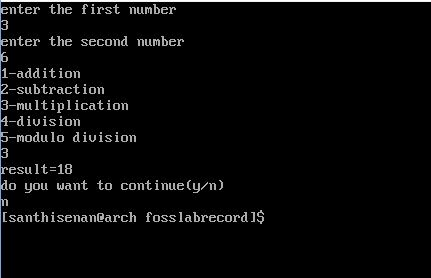
\includegraphics[width=\linewidth]{./outputs/simplecalcnew.jpg}
\end{figure}


\subsection{Result}
The shell script for a simple menu driven calculator was made and the output was verified. The script was run in ArchLinux 4.10.11 and screenshot of output is attached above.

\begin{refsection}
\cite{shellbible}
\cite{shellbook}
\printbibliography
\end{refsection}

\newpage

\section{Script that accepts two arguments from the commad line and operates on them}
\subsection{Aim}
Write a script called addnames that is to be called as follows ./addnames ulist username
Here ulist is the name of the file that contains list of user names and username is a particular student's username. The script should
\begin{itemize}
\item check that the correct number of arguments was received and print a message, in case the number of arguments is incorrect
\item check whether the ulist file exists and print an error message if it does not
\item check whether the username already exists in the file. If the username exists, print a message stating that the name already exists. Otherwise, add the username to the end of
the list.
\end{itemize}

\subsection{Shell script}
\begin{verbatim}

#!/bin/bash
if [ $# -eq 2 ];
then
    if [ ! -f ~/classlist ] || [ $1 != "classlist" ];
    then 
        echo "file not found"
    else
        count="$(grep $2 ~/classlist | wc -l)"
        if [ $count -eq 0 ];
        then 
            echo $2 >> ~/classlist
            echo "The new claslist is "
            cat ~/classlist
        else
            echo "Name already exists in the file"
            cat ~/classlist
        fi
    fi
else
    echo "Enter the correct number of arguments : ./addnames.sh classlist
    username"
fi

\end{verbatim}

\subsection{Output}
\begin{figure}[h!]
	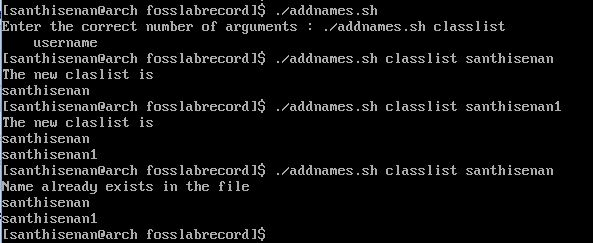
\includegraphics[width=\linewidth]{./outputs/addnamesnew.jpg}
\end{figure}


\subsection{Result}
The required shell script was made and the output was verfied. The script was run on ArchLinux 4.10.11.

\begin{refsection}
\cite{shellbible}
\cite{shellbook}
\printbibliography
\end{refsection}

\newpage

\section{Version Control System setup and usage using Git}

\subsection{Aim}
Version Control System setup and usage using GIT. Try the following features.
\begin{itemize}
\item Creating a repository
\item Checking out a repository
\item Adding content to the repository
\item Committing the data to a repository
\item Updating the local copy
\item Comparing different revisions
\item Revert
\item Conflicts and a conflict Resolution
\end{itemize}

\subsection{Theory}
\begin{itemize}
\item Git

Git is free and open source version control system, originally created by Linus Torvalds in 2005. Version control systems (VCS) are a category of software tools that help software teams maintain their source code. VCS allows developers to keep track of every modification made to the source code and also to turn back the clock and compare the earlier versions of code to fix their mistakes.

\item Benefits of using a Version Control System
\begin{itemize}
\item A complete long term history of every files.
\item Branching and merging
\item Traceability - being able to trace every change made in the software and connect it to project management and bug tracking softwares
\end{itemize}

\item Creating a repository

You can use the UI provided by websites to create a repository and clone the repository to the local computer. 

To clone an existing repository use \textit{git clone https://example\_url.git} .

Use the command git init when inside your project?s home folder to initialise an empty repository.

\item Basic Git commands
\begin{table}[htb]
\caption{Basic Commands}

\label{Basic commands in Git}
\begin{tabular}{|p{7cm}|p{7cm}|}
\noalign{\smallskip} \hline \hline \noalign{\smallskip}
Command & Use\\
\hline
git init & create a new repository\\
git clone $<$repo$>$& clone the repository on to the local machine\\
git status &get the status of your local repository. It tells you how your project is progressing when compared to the remote repository\\
git add $<$filename$>$ & tell git to start tracking the file\\
git add . & add all files\\
git commit  & commits all the added files. You must provide a commit message in the text editor that opens up\\
git commit -m"commit message" & a commit command with the message\\
git push origin master & save the committed changes to server\\
git pull -all & pull all changes from bitbucket server to your local repository\\
\noalign{\smallskip} \hline \hline \noalign{\smallskip}
\end{tabular}
\end{table}


\item Branching in Git

Branches are most powerful when you are working on a team. You can work on your part of the project by creating a branch and merging it to the main branch when you have finished. A brach provides an independent area for yourself to work.

There will be a main branch called master by default.

\begin{table}[htb]
\caption{Branching}
\begin{tabular}{|p{7cm}|p{7cm}|}
\noalign{\smallskip} \hline \hline \noalign{\smallskip}
Command & Use\\
\hline
git branch new\_branch & create a new branch \\
git checkout new\_branch & checkout to the new branch to start using it\\
git merge new\_branch & merge the new\_branch to the master branch (perform this operation after checking out to the master branch)\\
git branch -d branch\_name & delete a branch\\
\noalign{\smallskip} \hline \hline \noalign{\smallskip}
\end{tabular}
\end{table}

\item Forking 

You have only read access but not write access to another user?s repository.This is where the concept of forking comes in.
Here is the process of forking a repository

\begin{itemize}
\item Fork the repository to copy it to your account.
\item Clone the forked repository to your local computer
\item Make changes in the repository
\item Push the changes to your repository
\item Create a PULL REQUEST from the original repository you forked and add the changes you have made
\item Wait for the owner of the original repository to accept or reject changes
\end{itemize}

To fork a repository use the website of the git client you are using.

\item Undoing changes in a repository
\begin{itemize}
\item    the git checkout command serves three distinct functions - checking out files , checking out commits , checking out branches

Checking out a commit makes the entire working directory match that commit. This can be used to view an old state of your project without altering the current state in any way.

How to use checkout

\hspace{10mm} \textit{git log --oneline} will show the ID of each commit made 

\hspace{10mm} use textit{git checkout $<$commit\_id$>$} to go to that commit

\item git revert

\hspace{10mm} git revert $<$commit$>$ can also be used to undo changes. 

\hspace {10mm} This generates a new commit that undoes all of the changes introduced in $<$commit$>$  and apply it to the current branch

\item git reset

\hspace{10mm} git reset <file> is used to remove the file from staging area but leave the working directory unchanged. This unstages a file without overwriting any changes

\hspace{10mm} git reset is used to reset the staging area to match the most recent commit, but leave the working directory unchanged.

\hspace{10mm} git reset - - hard is used to reset the staging area and the working directory to match the most recent commit.  The - - hard tag tells git to overwrite all changes in the working directory.

\hspace{10mm} git reset $<$commit$>$ Move the current branch tip backward to $<$commit$>$ , reset the staging area to match, but leave the working directory alone.

\hspace{10mm} git reset - - hard <commit> moves the branch tip backwards to $<$commit$>$ and resets both the staging area and working directory to match.


\end{itemize}


\item Managing Conflicts

\begin{itemize}
\item When an user rebases or merges conflicts may occur. Conflicts occur when git cannot merge or rebase properly.
\item If a merge conflict occurs, we have to resolve the conflict in order to move forward with the merge/rebase
\item Run a git status to see where the problem is.
\item Edit the file to resolve the conflict.
\item Add the files again and use git rebase - - continue
\item If you are not able to resolve the conflict, use git rebase - - abort to abort the rebase.(similarly abort the merge)
\item Use git push origin master to push the changes
\end{itemize}

\item Comparing Different Revisions

\hspace{10mm} git diff $<$commit$>$ $<$commit$>$ can be used to compare two different commits

\hspace{10mm} here the $<$commit$>$ is the commit id of the specific commit

\end{itemize}

\subsection{Result}

Basic git operations were familiarised. All the opreations were performed in Git 2.10.1. Check out this repository in Github - https://github.com/santhisenan/fosslabrecord.git.

\begin{refsection}
\cite{gitdoc}
\cite{gitdoc1}
\printbibliography
\end{refsection}
\newpage
\section{Shell script which starts on system boot up and kills every process which uses more than a specified amount of memory or CPU}

\subsection{Aim}
Shell script which starts on system boot up and kills every process which uses more than a specified amount of memory or CPU.

\subsection{Shell Script}
\begin{verbatim}
#!/bin/sh
memlimit=10.0;
cpulimit=10.0;
while(true)
do
echo "script running.."
ps -e -o pmem=,pcpu=,pid=,user=,comm= | sort=-pmem |
while read size cpu pid user comm
do 
kill_mem=0
kill_cpu=0
if [ "$user" = "santhisenan" ]
then
    echo "Script Running..."
    kill_mem=` echo "$size>$memlimit" | bc `
    kill_cpu=` echo "$cpu>$cpulimit" | bc `
    if [ "$kill_mem = 1" ]
    then
        echo "process with PID $pid killed"
        kill $pid
    elif [ "$kill_cpu = 1" ]
    then
        echo "process with PID $pid killed"
        kill $pid
    else
    continue
    fi
fi
done
sleep 1
done

\end{verbatim}

\subsection{Output}
\begin{figure}[h!]
	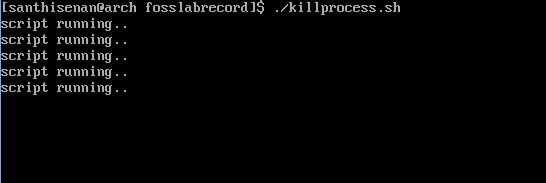
\includegraphics[width=\linewidth]{./outputs/killprocessnew.jpg}
\end{figure}

\subsection{Result}
A shell script for killing processes that consume more than a specific amount of memory and cpu was made and the output was verified. The shell script was run on ArchLinux 4.10.11.

\begin{refsection}
\cite{shellbible}
\cite{shellbook}
\printbibliography
\end{refsection}

\newpage
\section{Simple Text Processing using Perl and Awk}

\subsection{Aim}
Perform simple text processing using Perl, Awk.

\subsection{Script}

\begin{verbatim}
print("Please enter a string on which you would like to perform the regular expression operations\n");
$a=<>;
$c=0;
while ($c==0)
{
	print("Please enter the Regular expression to be evaluated\n");
	$b=<>;
	@regex=split("",$b);
	if ($regex[0] eq "m")
	{
		print ("The regular expression entered is a match operator\n");
		$len=length $b;
		$b=substr $b,2,$len-4;
		if($a=~$b)
		{
			print("There is a match found in the input string\n");
		}
		else
		{
			print ("There is no match found in the input string\n");
		}
	}
	elsif ($regex[0] eq "s")
	{
		print ("The regular expression is a substitute operator\n");
		$i=2;
		$t1="";
		for ($i=2;$i<length $b;$i=$i+1)
		{
			if($regex[$i] eq '/')
			{
				last;
			}
			else
			{
				$t1=$t1.$regex[$i];
			}
		}
		$i=$i+1;
		$t2="";
		for ($r=$i;$r<length $b;$r=$r+1)
		{
			if($regex[$r] eq '/')
			{
				last;
			}
			else
			{
				$t2=$t2.$regex[$r];
			}
		}
		$a=~s/$t1/$t2/;
		print ("The contents of the string now is $a\n");
	}
	elsif($regex[0] eq 't' && $regex[1] eq 'r')
	{
		print ("The regular expression if a translate operator\n");
		$i=3;
		$t1="";
		for ($i=3;$i<length $b;$i=$i+1)
		{
			if($regex[$i] eq '/')
			{
				last;
			}
			else
			{
				$t1=$t1.$regex[$i];
			}
		}
		$i=$i+1;
		$t2="";
		for ($r=$i;$r<length $b;$r=$r+1)
		{
			if($regex[$r] eq '/')
			{
				last;
			}
			else
			{
				$t2=$t2.$regex[$r];
			}
		}
		$a=~tr/$t1/$t2/;
		print ("The current contents of the string are $a\n");
	}
	print("Enter 0 if you would like to continue with the program, Enter 1 to exit from the program\n");
	$c=<>;
}
\end{verbatim}

\subsection{Result}
The script for simple word processing was made and the output was verified.

\begin{refsection}
\cite{perlbook}
\cite{perlweb}
\printbibliography
\end{refsection}

\newpage
\section{Running PHP}

\subsection{Aim}
Running PHP : simple applications like login forms after setting up a LAMP stack.

\subsection{Installing LAMP stack}
\begin{itemize}
\item Install Apache

To install Apache you must install the Metapackage apache2. This can be done by searching for and installing in the Software Centre, or by running the following command.

\textit{sudo apt-get install apache2}

\item Install MySQL

To install MySQL you must install the Metapackage mysql-server. This can be done by searching for and installing in the Software Centre, or by running the following command.

\textit{sudo apt-get install mysql-server}

\item Install PHP

To install PHP you must install the Metapackages php5 and libapache2-mod-php5. This can be done by searching for and installing in the Software Centre, or by running the following command.

\textit{sudo apt-get install php5 libapache2-mod-php5}

\item  Restart Server

Your server should restart Apache automatically after the installation of both MySQL and PHP. If it doesn't, execute this command.

\textit{sudo /etc/init.d/apache2 restart}

\item Check Apache

Open a web browser and navigate to http://localhost/. You should see a message saying It works!

\textit{sudo apt-get install mysql-server}

\item Install MySQL

To install MySQL you must install the Metapackage mysql-server. This can be done by searching for and installing in the Software Centre, or by running the following command.

\textit{sudo apt-get install mysql-server}

\item Check PHP

You can check your PHP by executing any PHP file from within /var/www/. Alternatively you can execute the following command, which will make PHP run the code without the need for creating a file .

\textit{php -r 'echo "$\backslash$n$\backslash$nYour PHP installation is working fine.$\backslash$n$\backslash$n$\backslash$n";'}

 
\end{itemize}

\subsection {PHP Example - Login From files}
\begin{itemize}
\item config.php

\begin{verbatim}
<?php 
define('DB_SERVER','localhost');
define('DB_USERNAME','fc');
define('DB_PASSWORD','');
define('DB_DATABASE','fossdb');
$db = mysqli_connect(DB_SERVER,DB_USERNAME,DB_PASSWORD,DB_DATABASE);
 ?>
\end{verbatim}

\item login.php

\begin{verbatim}

<?php 

include('config.php');

session_start();

$error="";

if($_SERVER["REQUEST_METHOD"] == "POST"){
	  $myusername =$_POST['username'];
    $mypassword = $_POST['password'];
    $sql = "SELECT * FROM admin WHERE username = '$myusername' and password = '$mypassword'";
      $result = mysqli_query($db,$sql) or die(mysqli_error($db));;
      $row = mysqli_fetch_array($result,MYSQLI_ASSOC);
      $count = mysqli_num_rows($result);

      if($count == 1) {
        session_register("myusername");
         $_SESSION['username'] = $myusername;
         $_SESSION['loggedin'] = true;

         // header('Location: http://localhost/login/welcome.php');
         // exit;
         error_reporting(E_ALL | E_WARNING | E_NOTICE);
ini_set('display_errors', TRUE);


flush();
header("Location:http://localhost/login/welcome.php");
die('should have redirected by now');

      }
      else {
         $error = "Your Login Name or Password is invalid";
      }


}

 ?>

<html>	
<head>
	<title>Login Page</title>
</head>
<div><?php echo $error ?></div>
<body>
	<form action="login.php" method="POST">
		<input type="text" placeholder="username" name="username">
		<input type="password" placeholder="password" name="password">
		<input type="submit" value="submit">

	</form>
</body>


 </html>
 
\end{verbatim}

\item session.php

\begin{verbatim}
<?php
   include('config.php');
   session_start();
   
   $user_check = $_SESSION['username'];
   
   $ses_sql = mysqli_query($db,"select username from admin where username = '$user_check' ");
   
   $row = mysqli_fetch_array($ses_sql,MYSQLI_ASSOC);
   
   $login_session = $row['username'];
   
   if(!isset($_SESSION['login_user'])){
      header("location:login.php");
   }
?>
\end{verbatim}

\item welcome.php

\begin{verbatim}
<html>
	<body>
		Logged in
	</body>
</html>
\end{verbatim}

\end{itemize}
\subsection{Result}
LAMP stack was successfully installed and a sample login form using PHP and mysql was made.

\begin{refsection}
\cite{lamp}
\printbibliography
\end{refsection}


\newpage
\section{GUI Programming}

\subsection{Aim}
 Create scientific calculator using GTK
 
 
 
 










	




























\end{document}                       
